\chapter{Special Relativity: Frames, Simultaneity, and the Lorentz Transformation}

Relativity is the principle that the laws of physics do not depend on which inertial frame we use to describe them. Our first task is kinematics: the meaning of space, time, motion, synchronization, and the transformation from one inertial frame to another. Dynamics comes afterward, with relativistic energy, momentum, force, the analog of Newton's equation of motion, and the meaning of \(E=mc^2\). Once that structure is secure, we can approach general relativity conceptually through curved spacetime, the motion of particles in a prescribed gravitational field, black holes, and the expansion of the universe, without beginning from the difficult problem of solving Einstein's field equations.

The distinction between conceptual and mathematical rigor is worth making. We will not use an approximation that is knowingly false. Rather, we will emphasize what a gravitational field does to clocks, particles, and geometry while postponing the machinery needed to construct arbitrary solutions of the field equations. Special relativity must be treated more explicitly because all of that later reasoning rests on its kinematics.

The right place to start is therefore not with a celebrated formula, but with a precise account of what an observer means by a place and a time.

\section{A Frame Is a Physical Coordinate System}

Imagine space filled with an arbitrarily fine lattice of meter sticks. Every lattice point is labeled by three spatial coordinates, and at every point there is a clock. Together the rods and clocks constitute a reference frame.

\begin{definition}
An \emph{event} is something that happens at one place and one time. In one spatial dimension its coordinates are written \((x,t)\); in three dimensions they are \((x,y,z,t)\).
\end{definition}

Newtonian physics adds a powerful assumption: all ideal clocks can be synchronized once and for all. Time is universal. A clock may be moved, and an observer may carry a watch, but everyone is supposed to agree on the same \(t\) everywhere. This is sometimes called absolute time; one may picture it as God's time, a single clock for the whole world.

The principle of relativity is older than Einstein. Its natural picture is a train moving so uniformly over perfectly smooth rails that nothing rattles or shakes. Inside the train we may toss and catch balls exactly as we do in a train standing at the station. Juggling is a surprisingly complete little mechanics experiment: it requires timing, gravity, alignment, and repeated control of trajectories. If the train moves at constant velocity, none of those rules changes. A ball thrown straight upward comes back to the same hand; the train does not slide out from under it. Galileo recognized this fact, and Newton expressed it systematically in his laws of motion.

Before Galileo, it was tempting to reason that the moving train ought to advance while the ball is in the air, forcing the juggler to reach backward or forward to recover it. The mistake is to forget that the ball already shares the train's horizontal velocity when it leaves the hand. No experiment confined to the smoothly moving carriage reveals a special state of absolute rest. Only relative motion between the two trains is observable.

The stationary train and the uniformly moving train are therefore two inertial frames. Before Einstein, they were related by Galilean transformations.

\section{Drawing Spacetime}

We suppress \(y\) and \(z\) for the moment and draw time vertically and position \(x\) horizontally. Every point in the drawing is an event. The line \(x=0\) is the history, or \emph{worldline}, of the spatial origin. The neighboring vertical lines \(x=1,2,3,\ldots\) are the worldlines of the other lattice points. Horizontal lines are sets of events with a common time.

\begin{figure}[H]
\centering

\includegraphics[width=0.62\textwidth]{lecture_01_figure_02.png}
\caption{The rest-frame time axis and the first worldlines of the spatial lattice.}
\lectureframe{00:16:38}
\end{figure}

The same construction is clearer in an idealized drawing:

\begin{figure}[H]
\centering
\begin{tikzpicture}[scale=0.95]
\draw[->] (-1.2,0) -- (5.2,0) node[right] {$x$};
\draw[->] (0,-0.2) -- (0,4.8) node[above] {$t$};
\foreach \x in {-1,1,2,3,4}
  \draw[gray!65] (\x,0) -- (\x,4.4);
\foreach \y in {1,2,3,4}
  \draw[gray!65] (-1.0,\y) -- (4.4,\y);
\fill (0,0) circle (1.5pt);
\node[below left] at (0,0) {$0$};
\node[left] at (0,1) {$1$};
\node[left] at (0,2) {$2$};
\node[left] at (0,3) {$3$};
\node[below] at (1,0) {$1$};
\node[below] at (2,0) {$2$};
\node[below] at (3,0) {$3$};
\end{tikzpicture}
\caption{A stationary spacetime lattice. Vertical lines have constant position; horizontal lines have constant time.}
\end{figure}

The grid is imaginary, and its spacing is arbitrary. We can use meters, centimeters, microns, or any still smaller interval that makes physical sense. Its purpose is to assign a precise coordinate to every event.

The phrase "frame of reference" now has operational content. It is not merely a viewpoint or a person looking in some direction. It is an extended coordinate apparatus. Given an event, the local rods specify where it happened and the local clock specifies when. Other physical quantities can then be compared between frames: the position and velocity of a particle, its energy, perhaps the temperature of a body, and eventually its momentum and force. The simplest comparison is the one involving \(x\) and \(t\), so we begin there.

Now place a second lattice on a train moving in the positive \(x\)-direction with constant velocity \(v\). Choose the origins to coincide at \(t=0\). The moving origin then follows
\begin{equation}
x=vt.
\end{equation}
Every other point fixed in the train follows a parallel tilted worldline. The tilt is simply the geometric statement that the train changes position as time passes.

Suppose the train's rear point is the primed origin. At \(t=0\) it coincides with the station origin. At a later time \(t\), its stationary coordinate is \(vt\). A nearby event at coordinate \(x\) is therefore only \(x-vt\) from the train's origin. This is why the transformation is a subtraction rather than an arbitrary algebraic rule.

Let \((x,t)\) be the coordinates of an event in the station frame and \((x',t')\) its coordinates in the train frame. Galileo and Newton retain universal time,
\begin{equation}
t'=t.
\end{equation}
During the time \(t\), the moving origin advances by \(vt\), so the distance from that origin to the event is
\begin{equation}
x'=x-vt.
\end{equation}
Together,
\begin{align}
t'&=t, & x'&=x-vt.
\label{eq:galilean-forward}
\end{align}
Solving for the unprimed coordinates gives the inverse transformation,
\begin{align}
t&=t', & x&=x'+vt'.
\label{eq:galilean-inverse}
\end{align}

\begin{figure}[H]
\centering

\includegraphics[width=0.72\textwidth]{lecture_01_figure_03.png}
\caption{The Galilean transformation written beside the two spacetime lattices.}
\lectureframe{00:21:57}
\end{figure}

The first pair tells the moving observer how to translate coordinates supplied by the stationary observer. The inverse pair translates back. This reciprocal conversion between descriptions is the mathematical content of Galilean relativity.

The replacement \(t\to t'\) in the inverse spatial formula is harmless only because Galilean theory has already declared \(t=t'\). It is useful to notice that assumption now. In Einstein's theory the two time coordinates will differ, and such substitutions will no longer be automatic.

\begin{classroomqa}
\audiencequestion{If a clock is carried away and then brought back, how can we know that its motion did not first speed it up and then slow it down, concealing the effect when the clocks are compared?
\lecturetimestamp{00:23:09}}
\lecturerresponse{Galileo could not have established universal time with modern precision; it was a physical guess. We can test the guess in many ways: carry good clocks in opposite directions, repeat the trip north--south as well as east--west, move one clock around the other, or exchange timing signals without bringing the clocks together. At ordinary speeds all such tests agree to very high precision. With sufficiently accurate clocks or sufficiently large speeds, a small discrepancy does appear. That failure of universal time is not a defect in the experiment; it is one of the phenomena special relativity must explain.}
\end{classroomqa}

\section{Galilean Invariants and Newton's Law}

An invariant is a quantity on which all the inertial observers under discussion agree. Coordinates themselves need not be invariant. What matters is whether the laws assembled from them retain the same form.

The word is used both as a noun and an adjective. A number can be an invariant, and an equation can be invariant under a transformation. The distinction between invariant quantities and invariant laws prevents a common confusion: relativity does not claim that every observer obtains the same coordinate for everything. It claims that the physical law connecting their measurements has the same form.

Take two simultaneous events at positions \(x_1\) and \(x_2\). Equation~\eqref{eq:galilean-forward} gives
\begin{align}
x_1'&=x_1-vt,\\
x_2'&=x_2-vt.
\end{align}
Their separation is therefore
\begin{equation}
x_2'-x_1'=(x_2-vt)-(x_1-vt)=x_2-x_1.
\end{equation}
In Galilean physics, the distance between events occurring at the same time is invariant even though the individual positions are not.

\begin{classroomqa}
\audiencequestion{Are the two occurrences of \(t\) in that subtraction really the same time?
\lecturetimestamp{00:28:16}}
\lecturerresponse{Yes. We deliberately chose the two events to be \((x_1,t)\) and \((x_2,t)\). They lie on one horizontal constant-time line. The common term \(vt\) therefore cancels. If the events occurred at different times, this argument would not establish an invariant spatial separation.}
\end{classroomqa}

Now describe a particle by a trajectory \(x(t)\). The train observer assigns
\begin{equation}
x'(t)=x(t)-vt.
\end{equation}
Differentiating once gives the familiar addition rule for velocities,
\begin{equation}
\frac{dx'}{dt}=\frac{dx}{dt}-v.
\end{equation}
Position and velocity are frame-dependent. An observer moving alongside an arrow sees it travel more slowly than an observer standing beside the track.

Differentiate again. Since the relative velocity \(v\) is constant,
\begin{equation}
\frac{d^2x'}{dt^2}=\frac{d^2x}{dt^2}.
\end{equation}
Acceleration is invariant under a Galilean transformation. This strongly suggests why Newton's law is written in terms of acceleration rather than position or velocity.

This is the acceleration of an observed object, not the acceleration of the train observer. Both frames are inertial, so neither frame accelerates relative to the other. Objects may accelerate left or right inside either description, and the two observers agree on the value of that acceleration even though they disagree on the object's position and velocity.

Suppose two particles exert a force on one another and the force depends only on their simultaneous separation. That separation is invariant, so the force is invariant. If mass is also an intrinsic, frame-independent property, then every inertial observer can write
\begin{equation}
F=ma
\end{equation}
in exactly the same form. Newtonian mechanics is invariant under Galilean transformations. It is not merely plausible; throughout the domain of ordinary speeds it is extraordinarily accurate.

The argument applies to familiar central forces such as Newtonian gravity or electrostatics, where the magnitude is a function of distance. Since all Galilean observers agree on that distance at a common time, they agree on the force. With force and acceleration fixed, consistency then requires them to agree on mass as well: a one-kilogram object remains a one-kilogram object when carried past on a train. Every symbol in \(F=ma\) fits the same invariant structure.

\section{Light Does Not Fit the Galilean Rule}

Electromagnetism creates the difficulty. Maxwell's equations predict waves that travel through empty space with a definite speed \(c\). If Maxwell's equations are laws of nature and the laws of nature are the same in every inertial frame, then all inertial observers must obtain the same \(c\).

Galilean kinematics predicts something else. A right-moving light pulse in the stationary frame satisfies
\begin{equation}
x=ct.
\end{equation}
Applying the spatial transformation gives
\begin{equation}
x'=x-vt=(c-v)t.
\end{equation}
Because \(t'=t\), the train observer would measure the speed \(c-v\).

The contradiction can be stated sharply. If Maxwell's equations retain their form, they predict \(c\) in the primed frame. If the Galilean transformation is retained, it predicts \(c-v\). Both cannot be exact when \(v\ne0\).

This result looks perfectly natural if light behaves like an ordinary wave in a medium. A boat moving with a water wave measures a lower relative wave speed. A listener moving through still air measures a sound speed shifted by the listener's motion relative to the air. Nineteenth-century physicists were therefore led toward a preferred state of rest, an ether frame in which Maxwell's equations would have their simplest form and light would move at \(c\). Experiments designed to detect motion relative to such a preferred frame found no corresponding effect.

There were several possible experimental arrangements, but their common aim was to compare light propagation for observers in different states or directions of motion. None revealed the expected Galilean shift. The failure was not a small technical nuisance. It forced a choice among the relativity principle, Maxwell's equations, and the inherited notions of space and time.

Einstein approached the conflict more directly. As a young man he imagined chasing a light wave. If he could catch up with it, its oscillating electromagnetic pattern would stand frozen in space, yet Maxwell's equations allow no such stationary light wave. He chose to treat Maxwell's theory and the relativity principle as fundamental, then reconsider the assumptions hidden in our coordinates.

The reconstruction rests on two postulates:
\begin{enumerate}
\item The laws of physics have the same form in every inertial frame.
\item Light in vacuum has the same speed \(c\) in every inertial frame.
\end{enumerate}

The second postulate cannot coexist with the Galilean transformation. Something deeper than the rule for adding velocities must change. Einstein's economical choice is to keep the two postulates and reconsider the apparently innocent Galilean equation \(t'=t\).

\section{Synchronizing Distant Clocks}

Spatial distances can be laid out with rods, but distant clocks require a synchronization convention. Put two clocks at equal distances from a midpoint observer. When each endpoint clock reads the appointed time, let it emit a flash. If the two flashes reach the midpoint together, call the endpoint clocks synchronized. If one flash arrives first, adjust the corresponding clock and repeat the procedure.

The word \emph{midpoint} is defined using the rods already laid out in that frame. The test therefore contains two separate ingredients: equal spatial distance from the endpoints and equal arrival time of the signals. Neither ingredient may be dropped. Repeating the procedure throughout the lattice supplies the horizontal constant-time lines that Newton had simply assumed.

This definition uses light because the postulate assigns light the same speed in every inertial frame. Once all neighboring pairs have been treated in this way, the entire lattice carries a synchronized family of clocks.

Now let a second lattice move through the first. The midpoint of the moving apparatus remains halfway between its two moving endpoints in its own frame. Relative to the stationary apparatus, however, it moves toward one incoming flash and away from the other. Flashes emitted simultaneously according to the stationary clocks do not arrive together at the moving midpoint. Since the moving observer applies the same midpoint-and-light rule, that observer cannot call those emissions simultaneous. Each frame synchronizes its own clocks consistently, but the two synchronizations disagree.

This is not an optical illusion produced by the finite travel time of light. Each observer knows that light takes time to arrive and corrects for it using the same speed \(c\). The disagreement remains after that correction because the observers do not select the same distant events as a simultaneous pair. Simultaneity itself, rather than merely the appearance of simultaneity, is relative.

\begin{classroomqa}
\audiencequestion{Could we avoid this conclusion by synchronizing clocks with sound instead of light?
\lecturetimestamp{00:49:03}}
\lecturerresponse{Sound works as a synchronization signal in a frame where the air is at rest, but its measured speed is not the same in every inertial frame. An open train moving through still air is moving relative to the sound-carrying medium, so forward and backward sound signals do not behave symmetrically there. Light is different by postulate: there is no detectable optical medium whose rest frame selects one observer. We therefore use light and follow the consequences.}
\end{classroomqa}

The qualitative disagreement is clear. We now calculate exactly which events the moving observer calls simultaneous.

\section{The Light-Ray Construction}

For the construction it is convenient to choose units in which
\begin{equation}
c=1.
\end{equation}
One unit of distance is then the distance light travels in one unit of time: light-seconds paired with seconds, or light-years paired with years. Space and time carry the same units, velocities are dimensionless, and light rays appear at \(45^\circ\). A right-moving ray has
\begin{equation}
x=t+d,
\end{equation}
while a left-moving ray has
\begin{equation}
x=-t+d'.
\end{equation}
The two rays through the origin are simply \(x=t\) and \(x=-t\). Timelike trajectories, belonging to objects slower than light, lie closer to the vertical axis. A hypothetical superluminal trajectory would lie closer to the horizontal axis.

The angle in the drawing is meaningful only after this unit choice. In meters and seconds, a light ray would look almost horizontal because it covers roughly \(3\times10^8\) meters in one second. Choosing light-seconds for distance rescales the horizontal axis and makes the causal geometry visible.

Consider three parallel worldlines in the moving lattice,
\begin{equation}
x=vt,\qquad x=vt+L,\qquad x=vt+2L.
\label{eq:moving-worldlines}
\end{equation}
The middle worldline belongs to the observer who tests simultaneity between the two outer points. All three points move uniformly and preserve their relative arrangement in the primed frame.

\begin{figure}[H]
\centering

\includegraphics[width=0.72\textwidth]{lecture_01_figure_04.png}
\caption{The forward light ray \(x=t\) meeting the middle moving worldline.}
\lectureframe{01:02:33}
\end{figure}

The complete geometry can be drawn without the obstruction of a person standing at the board:

\begin{figure}[H]
\centering
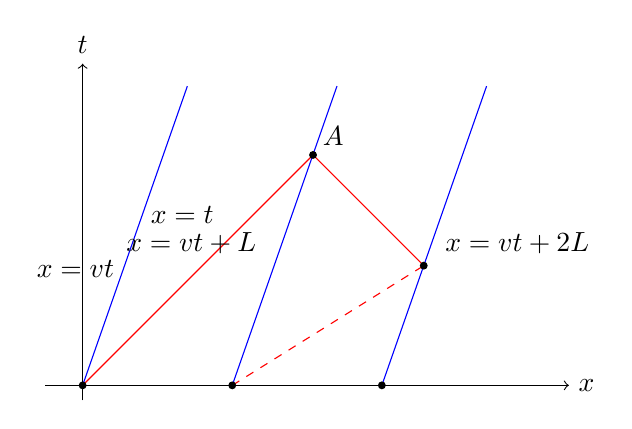
\begin{tikzpicture}[scale=0.95]
\draw[->] (-0.5,0) -- (6.5,0) node[right] {$x$};
\draw[->] (0,-0.2) -- (0,4.3) node[above] {$t$};
\draw[blue] (0,0) -- (1.4,4.0);
\draw[blue] (2.0,0) -- (3.4,4.0);
\draw[blue] (4.0,0) -- (5.4,4.0);
\draw[red] (0,0) -- (3.08,3.08);
\draw[red] (3.08,3.08) -- (4.56,1.60);
\draw[red,dashed] (2.0,0) -- (4.56,1.60);
\fill (0,0) circle (1.5pt);
\fill (2.0,0) circle (1.5pt);
\fill (4.0,0) circle (1.5pt);
\fill (3.08,3.08) circle (1.5pt);
\fill (4.56,1.60) circle (1.5pt);
\node[left] at (0.55,1.55) {$x=vt$};
\node[left] at (2.45,1.9) {$x=vt+L$};
\node[right] at (4.72,1.9) {$x=vt+2L$};
\node[left] at (1.88,2.28) {$x=t$};
\node[above right] at (3.08,3.08) {$A$};
\end{tikzpicture}
\caption{Light signals determine the moving frame's line of simultaneity.}
\end{figure}

Send a right-moving light ray from the origin. Let \(A\) be its intersection with the middle worldline. The two equations at \(A\) are
\begin{align}
x&=t,\\
x&=vt+L.
\end{align}
Substitution gives
\begin{equation}
t=vt+L,
\end{equation}
and hence
\begin{equation}
t_A=x_A=\frac{L}{1-v}.
\label{eq:point-a}
\end{equation}

From \(A\), trace a left-moving light ray backward to the rightmost moving worldline. Its equation has the form
\begin{equation}
x+t=b.
\end{equation}
Because it passes through \(A\), Equation~\eqref{eq:point-a} fixes the constant:
\begin{equation}
b=x_A+t_A=\frac{2L}{1-v}.
\end{equation}
The backward ray therefore satisfies
\begin{equation}
x+t=\frac{2L}{1-v}.
\label{eq:backward-ray}
\end{equation}

Its intersection with the rightmost worldline follows from
\begin{align}
x+t&=\frac{2L}{1-v},\\
x&=vt+2L.
\end{align}
Eliminating \(x\),
\begin{align}
(1+v)t
  &=2L\left(\frac{1}{1-v}-1\right)\\
  &=\frac{2Lv}{1-v},
\end{align}
so
\begin{equation}
t=\frac{2Lv}{1-v^2}.
\end{equation}
Substitution into \(x=vt+2L\) gives
\begin{equation}
x=\frac{2L}{1-v^2}.
\end{equation}
The coordinates themselves are less important than their ratio:
\begin{equation}
\frac{t}{x}=v.
\end{equation}
Thus every event simultaneous with the origin according to the moving clocks lies on
\begin{equation}
t=vx,
\label{eq:simultaneity-c-one}
\end{equation}
whereas the moving origin follows
\begin{equation}
x=vt.
\label{eq:moving-time-axis}
\end{equation}
The two axes are tilted symmetrically around the \(45^\circ\) light ray.

All points on \(x=vt\) have the same primed position, \(x'=0\), while their primed times vary. All points on \(t=vx\) have the same primed time, \(t'=0\), while their primed positions vary. One line is therefore the primed time axis and the other the primed space axis. The long signal construction was needed to determine the second line; it could not be inferred from the moving worldline alone.

Restoring ordinary units in Equation~\eqref{eq:simultaneity-c-one} requires
\begin{equation}
t=\frac{v}{c^2}x.
\label{eq:simultaneity-dimensional}
\end{equation}
The factor \(c^2\) explains why the Newtonian picture works so well in daily life. For velocities tiny compared with \(c\), the slope of the moving simultaneity line is extremely small.

\begin{figure}[H]
\centering

\includegraphics[width=0.72\textwidth]{lecture_01_figure_05.png}
\caption{With \(c=1\), the primed time and simultaneity axes are symmetric about the light ray.}
\lectureframe{01:15:40}
\end{figure}

\begin{figure}[H]
\centering
\begin{tikzpicture}[scale=1.0]
\draw[->] (-2.2,0) -- (5.2,0) node[right] {$x$};
\draw[->] (0,-0.2) -- (0,4.9) node[above] {$t$};
\draw[red] (0,0) -- (3.9,3.9);
\draw[red] (0,0) -- (-1.8,1.8);
\draw[blue] (0,0) -- (1.8,4.5);
\draw[blue,dashed] (0,0) -- (4.5,1.8);
\node[right] at (3.9,3.9) {$x=t$};
\node[left] at (-1.8,1.8) {$x=-t$};
\node[above] at (1.8,4.5) {$x'=0$};
\node[right] at (4.5,1.8) {$t'=0$};
\end{tikzpicture}
\caption{The primed axes and invariant light rays in \(c=1\) units.}
\end{figure}

\section{Deriving the Lorentz Transformation}

The geometry fixes where each primed coordinate vanishes. Along the moving time axis \(x=vt\), we must have \(x'=0\). Along the moving simultaneity axis \(t=vx\), we must have \(t'=0\). The most general linear relations with those zero-sets can be written
\begin{align}
x'&=\frac{x-vt}{F(v)},\\
t'&=\frac{t-vx}{G(v)}.
\label{eq:fg-ansatz}
\end{align}
The factors \(F\) and \(G\) allow the primed coordinate scales to differ from the Galilean scales even though the axes have already been located. Linearity follows from the homogeneity of space and time: translating an experiment cannot change the transformation law.\editorialnote{This short linearity argument makes explicit an assumption used implicitly in the blackboard derivation.}

At this stage the geometry has told us a great deal but not everything. The numerators fix the tilt of the axes. They do not fix the unit spacing along those axes. That remaining scale information is exactly what \(F(v)\) and \(G(v)\) represent.

Now impose the invariance of light speed. A right-moving ray obeying \(x=t\) must also obey \(x'=t'\). Along that ray,
\begin{align}
x'&=\frac{(1-v)t}{F(v)},\\
t'&=\frac{(1-v)t}{G(v)}.
\end{align}
Equality for every point on the ray requires
\begin{equation}
F(v)=G(v).
\end{equation}
We may therefore write
\begin{align}
x'&=\frac{x-vt}{F(v)},\\
t'&=\frac{t-vx}{F(v)}.
\label{eq:common-f}
\end{align}

This step uses the first genuinely Einsteinian demand in the algebra. The same geometric line is a light ray for both observers, so the two primed coordinates must increase equally along it when \(c=1\). Different factors in the two equations would make the primed speed differ from unity.

One unknown function remains. Multiply Equation~\eqref{eq:common-f} by \(F(v)\):
\begin{align}
F(v)x'&=x-vt,\\
F(v)t'&=t-vx.
\end{align}
Multiplying the second equation by \(v\) and adding it to the first eliminates \(t\), giving
\begin{equation}
(1-v^2)x=F(v)(x'+vt').
\end{equation}
Similarly,
\begin{equation}
(1-v^2)t=F(v)(t'+vx').
\end{equation}
The inverse transformation is therefore
\begin{align}
x&=\frac{F(v)}{1-v^2}(x'+vt'),\\
t&=\frac{F(v)}{1-v^2}(t'+vx').
\end{align}

The principle of relativity makes the two frames reciprocal. If the station sees the train move at \(+v\), the train sees the station move at \(-v\). The inverse equations must consequently have the same form as the forward equations with the sign of \(v\) reversed. Their prefactors must satisfy
\begin{equation}
\frac{F(v)}{1-v^2}=\frac{1}{F(v)}.
\end{equation}
Hence
\begin{equation}
F(v)^2=1-v^2,
\end{equation}
and continuity with the identity transformation at \(v=0\) selects the positive root,
\begin{equation}
F(v)=\sqrt{1-v^2}.
\end{equation}

Nothing has been fitted to a particular light pulse. The result follows from the axes fixed by synchronization, the common speed of light, and the demand that neither inertial frame be privileged over the other.

The Lorentz transformation in units with \(c=1\) is
\begin{align}
x'&=\frac{x-vt}{\sqrt{1-v^2}},\\
t'&=\frac{t-vx}{\sqrt{1-v^2}}.
\label{eq:lorentz-c-one}
\end{align}
Its inverse is
\begin{align}
x&=\frac{x'+vt'}{\sqrt{1-v^2}},\\
t&=\frac{t'+vx'}{\sqrt{1-v^2}}.
\end{align}

\begin{figure}[H]
\centering

\includegraphics[width=0.76\textwidth]{lecture_01_figure_06.png}
\caption{The completed \(c=1\) Lorentz transformation on the blackboard.}
\lectureframe{01:32:38}
\end{figure}

The essential novelty is already visible in the time equation. Time is not simply carried unchanged from one frame to another. A primed time coordinate mixes unprimed time and position. Consequently \(t=\text{constant}\) and \(t'=\text{constant}\) describe different sets of events.

The mixing term is not an optional correction appended after the fact. Without it, the line \(t'=0\) would remain horizontal, distant simultaneity would stay universal, and the transformation could not preserve the speed of light.

\section{Restoring the Speed of Light and Checking the Result}

When \(c\ne1\), dimensional consistency restores the missing factors. The ratio \(v^2/c^2\) is dimensionless, while \((v/c^2)x\) has units of time. Thus
\begin{align}
x'&=\frac{x-vt}{\sqrt{1-v^2/c^2}},\\
t'&=\frac{t-(v/c^2)x}{\sqrt{1-v^2/c^2}}.
\label{eq:lorentz-dimensional}
\end{align}
The inverse is obtained by reversing the sign of \(v\):
\begin{align}
x&=\frac{x'+vt'}{\sqrt{1-v^2/c^2}},\\
t&=\frac{t'+(v/c^2)x'}{\sqrt{1-v^2/c^2}}.
\end{align}
Introducing
\begin{equation}
\gamma=\frac{1}{\sqrt{1-v^2/c^2}}
\end{equation}
would put these in the familiar compact form, but the denominator form keeps the derivation visible.

Numerically, \(c\simeq3\times10^8\,\mathrm{m/s}\), so \(c^2\simeq9\times10^{16}\,\mathrm{m^2/s^2}\). The large denominator makes both the simultaneity tilt and the factor \(v^2/c^2\) imperceptible in most mechanical experiments. Their smallness explains Galileo's success; it does not restore absolute time.

\begin{figure}[H]
\centering

\includegraphics[width=0.76\textwidth]{lecture_01_figure_07.png}
\caption{The Lorentz transformation after the factors of \(c\) have been restored.}
\lectureframe{01:35:58}
\end{figure}

Two checks are immediate. First take \(v\ll c\). Then \(v^2/c^2\) is negligible, and for ordinary distances the relativity-of-simultaneity term \(vx/c^2\) is also negligible. Equation~\eqref{eq:lorentz-dimensional} reduces to
\begin{equation}
t'\approx t,\qquad x'\approx x-vt.
\end{equation}
Galilean relativity is recovered as the low-speed approximation.

Second, test a light ray. Once \(c\) has been restored, a right-moving ray obeys \(x=ct\), not \(x=t\). Substitution gives
\begin{align}
x'&=\frac{(c-v)t}{\sqrt{1-v^2/c^2}},\\
t'&=\frac{(1-v/c)t}{\sqrt{1-v^2/c^2}}.
\end{align}
Since \(c-v=c(1-v/c)\),
\begin{equation}
x'=ct'.
\end{equation}
The primed observer measures the same speed \(c\). For a left-moving ray, substitution of \(x=-ct\) similarly gives
\begin{equation}
x'=-ct'.
\end{equation}
The transformation treats light moving in either direction correctly.

The distinction between \(x=t\) and \(x=ct\) is an instructive dimensional check. The former is correct only in units where \(c=1\). Restoring ordinary units in the transformation while leaving the ray equation in natural units would mix two conventions and produce a false result. Dimensional consistency catches the mistake immediately.

\section{The Midpoint Criterion}

\begin{classroomqa}
\audiencequestion{Suppose an observer receives two flashes at the same instant but is not halfway between their sources. May that observer conclude that the flashes were emitted simultaneously?
\lecturetimestamp{01:42:55}}
\lecturerresponse{No. Equal arrival times imply equal emission times only for the observer who is spatially midway between the two sources in the relevant frame. A receiver closer to one source can receive both flashes together even though the farther flash was emitted earlier. In the moving construction, the midpoint worldline \(x=vt+L\) is therefore essential. The forward ray \(x=t\) is followed until it meets that midpoint, and a backward light ray is then traced to \(x=vt+2L\). That second endpoint event, not an arbitrary equal-arrival event elsewhere, is simultaneous with the origin according to the moving frame.}
\end{classroomqa}

We have reached the complete coordinate transformation but not yet its most familiar consequences. Length contraction, time dilation, and proper time follow next, followed by relativistic momentum and energy. The foundation is already in place: each inertial frame may use the same laws and measure the same speed of light only because space and time mix, and because distant simultaneity belongs to a frame rather than to the world absolutely.
